\documentclass{article}

% Language setting
% Replace `english' with e.g. `spanish' to change the document language
\usepackage[english]{babel}


% Set page size and margins
% Replace `letterpaper' with `a4paper' for UK/EU standard size
\usepackage[a4paper,margin=2.5cm]{geometry}

% Header and footer Package
\usepackage{fancyhdr}

% Useful packages
\usepackage[colorlinks=true, allcolors=blue]{hyperref}
\usepackage{amsmath}
\usepackage{graphicx}
\usepackage{listings}
\usepackage{caption}
\usepackage{subcaption}
\usepackage{float}

\newcommand{\course}{Symmetric Key Cryptography}
\newcommand{\me}{João Gaspar (025605833A)}
\newcommand{\labName}{Lab 2. Enigma Cryptanalysis}


\fancyhead[L]{\course - \labName}
\fancyhead[R]{\me}
\pagestyle{fancy}
\title{\textit{\course} - \labName}
\author{\me}


\begin{document}
\maketitle
\section{Method of Batons}
The Method of Batons is a method that allows us to discover the initial position of the rotors, given that the attacker knows partially the plaintext associated to a specific ciphertext, this known part of the plaintext is called \textit{crib}.

This method can be applied whenever the machine has no plugboard, the rotors wirings and their turn points (the notches) alongside with the reflector wirings are known.
Whats kept unkown is the rest of the ciphertext and the used key.

To implement the method of the batons, we know that the machine can be modeled mathematically by:
\begin{equation}
    \left( c = N^{-1} Z N (p) \right)
    \label{eq:enigma}
\end{equation}

Where $N$ is the operator that model the moving rotors (\ref{eq:N}) and $Z$ is the operator that models the frozen rotors and the reflector, which constitutes as an involution.

\begin{equation}
    N = \prod_{k \in \text{Moving rotors}} P^{-i} R_k P^{i}
    \label{eq:N}
\end{equation}

We can rewrite (\ref{eq:enigma}) to
\begin{equation}
    \left( N(c) = Z N (p) \right)
    \label{eq:enigma2}
\end{equation}

Such that if we calculate both $N(p)$ and $N(c)$ for a rotor position, $Z$ can only be a proper involution iff. there is no contradiction, this means that if $Z(\alpha) = \beta \Leftrightarrow Z(Z(\alpha)) = Z(\beta) \Leftrightarrow \alpha = Z(\beta)$, and if does not apply to the $N(p) \leftrightarrow N(c)$ mapping, then it means that the tested rotor positions were not used to encrypt the plaintext, or the crib is not found at that spot. Nonetheless, I've disregarded the latter by implementing a solution that assumes that the tested crib is present in the beginning of the ciphertext.

With this in mind, I've implemented the solution where I pass through all of the first and second rotor positions (fig. \ref{fig:method}), since we cannot assume that the second rotor never turns, applied the operator $N$ to both the crib and the ciphertex (fig. \ref{fig:Noperator}) and created the $N(p) \leftrightarrow N(c)$ mappings (fig. \ref{fig:method}) to look for the first rotor positions where it created no inconsistencies.
I've also programmatically implemented this verification.

\begin{figure}[H]
    \begin{subfigure}[b]{0.60\textwidth}
        \centering
        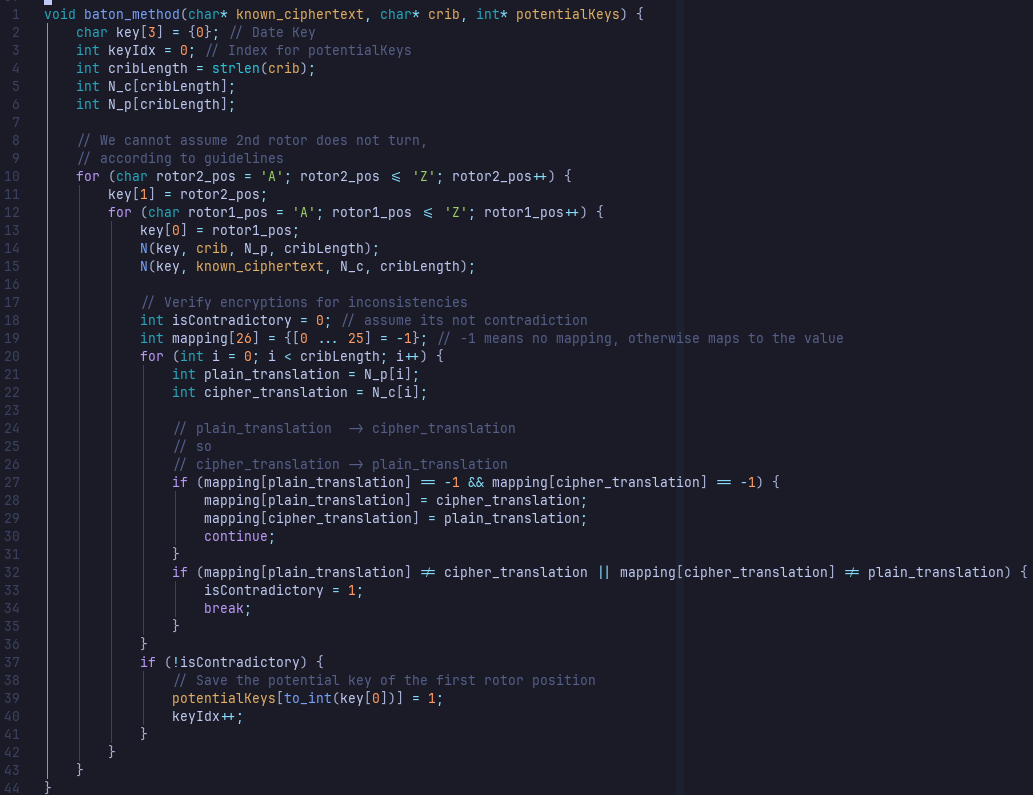
\includegraphics[width=\textwidth]{figures/ex1/batons_method}
        \caption{Method of Batons implementation}\label{fig:method}
    \end{subfigure}
    ~
    \begin{subfigure}[b]{0.40\textwidth}
        \centering
        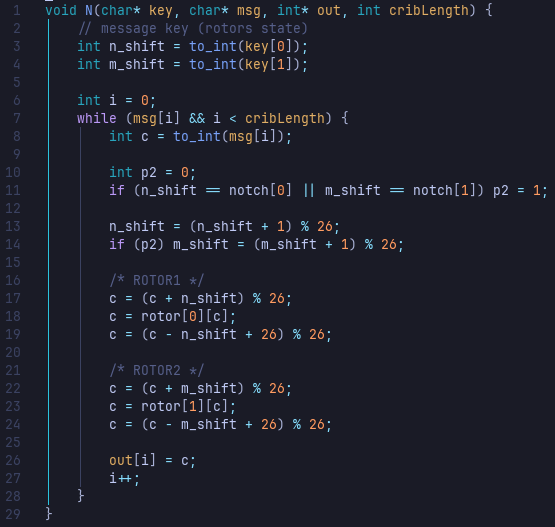
\includegraphics[width=\textwidth]{figures/ex1/N_operator}
        \caption{Implementation of the N operator}\label{fig:Noperator}
    \end{subfigure}
\end{figure}


By compiling and running, through the following command, I've reach the solution that with the crib THEREISN, the method can uniquely identify that the first rotor position was set to 'Q' at encryption.
\begin{lstlisting}[language=bash]
$ make ex1
gcc ex1_batons.c -o ex1_batons && ./ex1_batons ./exercise/1.txt THEREISN
Cyphertext to decrypt: ICUBWUYIWNFSLMFUWLPBBXTJXD
Potential first rotor position:
Q
\end{lstlisting}

\section{Turing-Welchman's Attack}
\subsection{On Cycles}
I was given the following data:
\begin{table}[H]
    \begin{center}
        \begin{tabular}[c]{| l | l | l | l | l | l | l | l | l | l | l | l | l | l | l | }
            \hline
            Enigma state & 1 & 2 & 3 & 4 & 5 & 6 & 7 & 8 & 9 & 10 & 11 & 12 & 13 & 14 \\
            \hline
            Ciphertext & V & Z & T & Z & U & C & T & T & I & P & G & J & O & B \\
            \hline
            Plaintext & Z & J & J & V & S & Z & V & V & T & C & U & T & F & R \\
            \hline
        \end{tabular}
    \end{center}
\end{table}


In the figure \ref{fig:graph}, we can see a sketch of the corresponding graph to the given data.
\begin{figure}[H]
    \begin{center}
        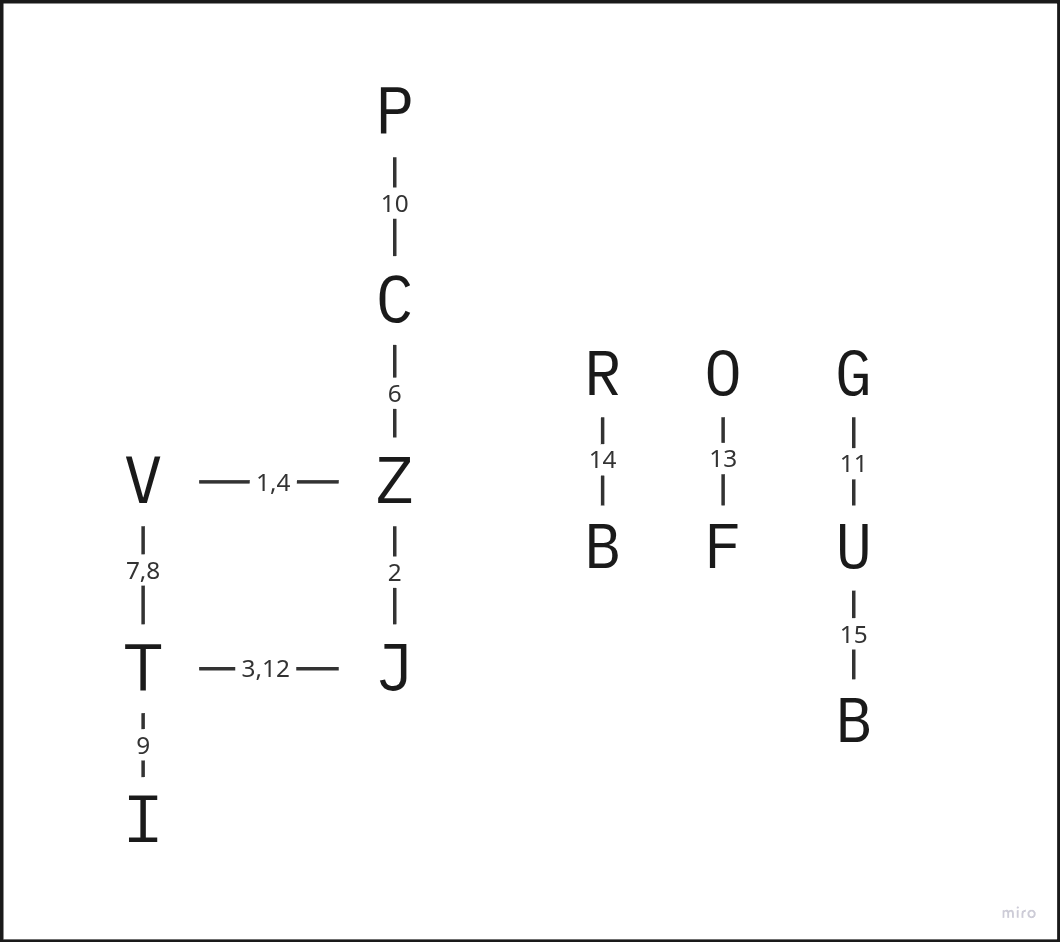
\includegraphics[width=0.45\textwidth]{figures/ex2/graph.png}
    \end{center}
    \caption{Connections' graph}\label{fig:graph}
\end{figure}

From this graph, I've derived the following equations:

\begin{equation}
    \begin{cases}
        C R_{1,4} C(V) = Z \\
        C R_2 C(Z) = J \\
        C R_{3,12} C(J) = T \\
        C R_{7,8} C(T) = V \\
    \end{cases}
    \label{eq:simpEq}
\end{equation}

These are the only important equations to us as any other equations don't help in finding meshes.
From these equations, I've derived the following four that will be our loops
\begin{equation}
    \begin{cases}
        R_1 R_2 R_3 R_7 C(V) = C(V) \\
        R_1 R_4 = C(V) \\
        R_7 R_{12} R_2 R_1 C(V) = C(V) \\
    \end{cases}
    \label{eq:LoopEqs}
\end{equation}
I've chosen these loops because none is in any way irrelevant since they are independent and because they all relate to the letter V simplifying the logic to be implemented in order to break the cipher.

The probability that a wrong guess survives on 3 independent loops is $\approx \frac{1}{26^3} = \frac{1}{17576}$, but since I test across 26 letters, the expected false positive rate per key is $\approx \frac{26}{26^3} = \frac{1}{26^2}$.
Across all keys, I would expectedly get $26^3 * \frac{1}{26^2} = 26$ candidate keys.

Given all my loops start at C(V) and end up at C(V), I assume so also in my implementation.

To implement the method:
\begin{enumerate}
    \item{Created the Enigma machines instances at position 0 until the biggest necessary position (12) [\ref{fig:enigmaInit}]}
    \item{Created Loop Objects with the encoded paths [\ref{fig:LoopObjs}]}
    \item{Iterating through all of the possible rotor positions and all loops do [\ref{fig:mainLoop}]:
        \begin{enumerate}
            \item For each letter calculate the character after passing through all the enigmas in the path of the loop
            \item {If the final result does not match the initial character then mark the letter as invalid}
            \item{After passing through all letters If there's not any valid encoding of the characters of the previous loop, skip to the next rotor position [\ref{fig:noPossible}]}
            \item{Otherwise print the possible plugboard configuration for the given key [\ref{fig:plugboard}]}
        \end{enumerate}
    }
\end{enumerate}

\begin{figure}[h]
    \begin{subfigure}[b]{0.45\textwidth}
        \centering
        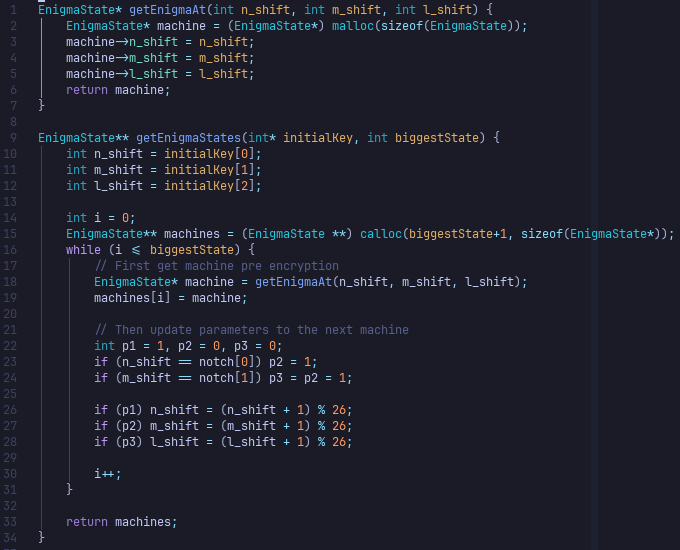
\includegraphics[width=\textwidth]{figures/ex2/enigmaInit.png}
        \caption{Enigma States initialization}\label{fig:enigmaInit}
    \end{subfigure}
    ~
    \begin{subfigure}[b]{0.50\textwidth}
        \centering
        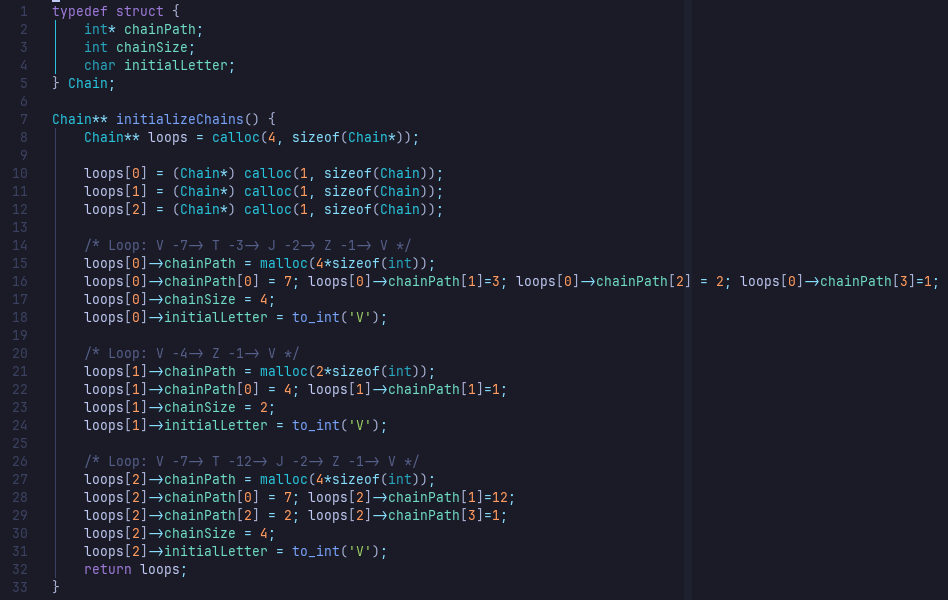
\includegraphics[width=\textwidth]{figures/ex2/LoopObjs.png}
        \caption{Encoding of the loops}\label{fig:LoopObjs}
    \end{subfigure}

    \begin{subfigure}[b]{0.45\textwidth}
        \centering
        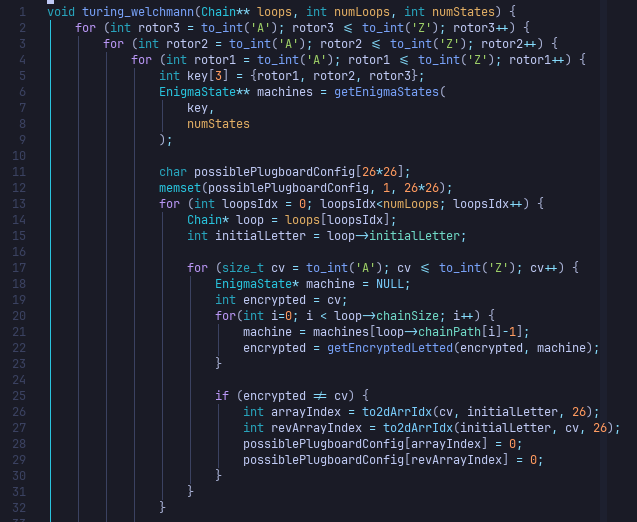
\includegraphics[width=\textwidth]{figures/ex2/mainLoop.png}
        \caption{Main Logic of the method}\label{fig:mainLoop}
    \end{subfigure}
    ~
    \begin{subfigure}[b]{0.50\textwidth}
        \centering
        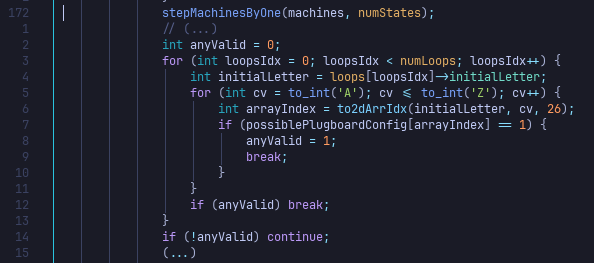
\includegraphics[width=\textwidth]{figures/ex2/noPossible.png}
        \caption{Discarding impossible dates}\label{fig:noPossible}
    \end{subfigure}

    \begin{subfigure}[b]{0.45\textwidth}
        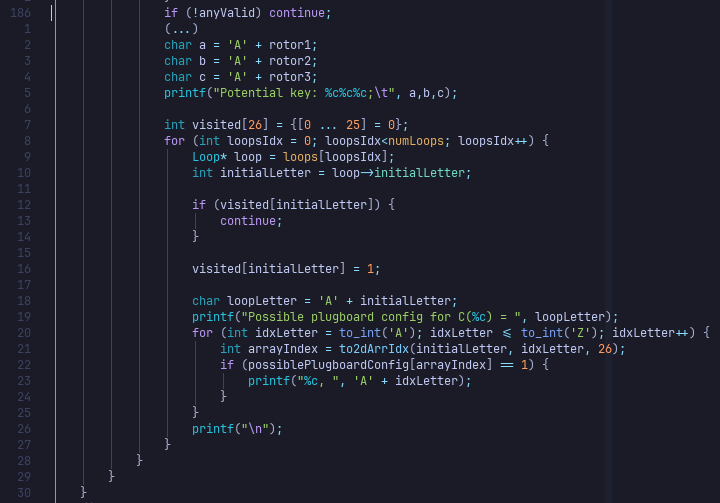
\includegraphics[width=\textwidth]{figures/ex2/plugboard.png}
        \caption{Output of possible plugboard config per key}\label{fig:plugboard}
    \end{subfigure}
\end{figure}


With this algorithm, I've got the following the following result on my loops:

\begin{lstlisting}[language=bash]
$ make ex2 && ./ex2_turing_loops
gcc ex2_turing_loops.c -g -O0 -o ex2_turing_loops
Potential key: BBA;     Possible plugboard config for C(V) = W, 
Potential key: MNB;     Possible plugboard config for C(V) = G, 
Potential key: DME;     Possible plugboard config for C(V) = F, 
Potential key: QPE;     Possible plugboard config for C(V) = B, 
Potential key: UZF;     Possible plugboard config for C(V) = N, 
Potential key: LZH;     Possible plugboard config for C(V) = L, 
Potential key: OEK;     Possible plugboard config for C(V) = I, 
Potential key: OFL;     Possible plugboard config for C(V) = I, 
Potential key: RRM;     Possible plugboard config for C(V) = X, 
Potential key: VVM;     Possible plugboard config for C(V) = O, 
Potential key: LZM;     Possible plugboard config for C(V) = S, 
Potential key: IJN;     Possible plugboard config for C(V) = Z, 
Potential key: LMP;     Possible plugboard config for C(V) = Z, 
Potential key: ZAQ;     Possible plugboard config for C(V) = J, 
Potential key: AMQ;     Possible plugboard config for C(V) = C, 
Potential key: CRR;     Possible plugboard config for C(V) = V, 
Potential key: KST;     Possible plugboard config for C(V) = J, 
Potential key: AWV;     Possible plugboard config for C(V) = D, 
\end{lstlisting}

So I got $18$ candidate keys, and expected $\approx 26$, So I assume that my calculations were indeed correct.
But I only know the translation of one letter on the plugboard per potential key, so also assume that I didn't understood correctly how either the method works, or how to get better results from it.
Nonetheless, we now have a way smaller keyspace to search with one entry of the plugboard per key; Significantly better than bruteforcing the solution from scratch.

\subsection{Implemebnting the Turing-Welchman Attack (no loops)}
To implement the Turing-Welchman attack, I used as the baseline the same code as before which I now know that although it looks like it works, it can be made better.
Nonetheless, the method is about propagating the constraints of the menu links through the diagonal board until no more elimination can be done, and then checking if any of the menu nodes have no possible options left, if so, discard the key, otherwise report it as a potential key.

So, by steps and without repeating the same logic as before, the method is as follows:
\begin{enumerate}
    \item {Created the chain of letters alongside the links between them, and the machines associated with each link. Which was the main step that could be improved if I didn't kept the same code as before as it required extra steps especially in the beginning of the \textit{Function turing\_welchman}. (Code is too big for a picture, please refer to \textit{Function initializeChains})}
    \item {For all keys, followed all the loops and for each loop and letter $\alpha$ discarded all the values of $\alpha=C(\text{Initial Letter})$ that didn't map back to $\alpha$ after going through the loop. [\ref{fig:loopElimination}]}
    \item {Welchman Diagonal Board:
        \begin{enumerate}
            \item {For each menu link $A \xrightarrow{state_i} P$, propagate the constraint $C(A)=x \Rightarrow C(B)=enc(x)$ and its reverse $C(B)=y \Rightarrow C(A)=enc(y)$ through the diagonal board until no more elimination can be done [\ref{fig:welchman}].}
            \item {Afterwards, check if any of the menu nodes have no possible options left, if so, discard the key, otherwise save it as a potential key [\ref{fig:potentialKeys}].}
        \end{enumerate}
    }
    \item {Finally, print the potential keys and their possible plugboard configurations [\ref{fig:finalOutput}].}
\end{enumerate}

\begin{figure}[H]
    \begin{subfigure}[b]{0.45\textwidth}
        \centering
        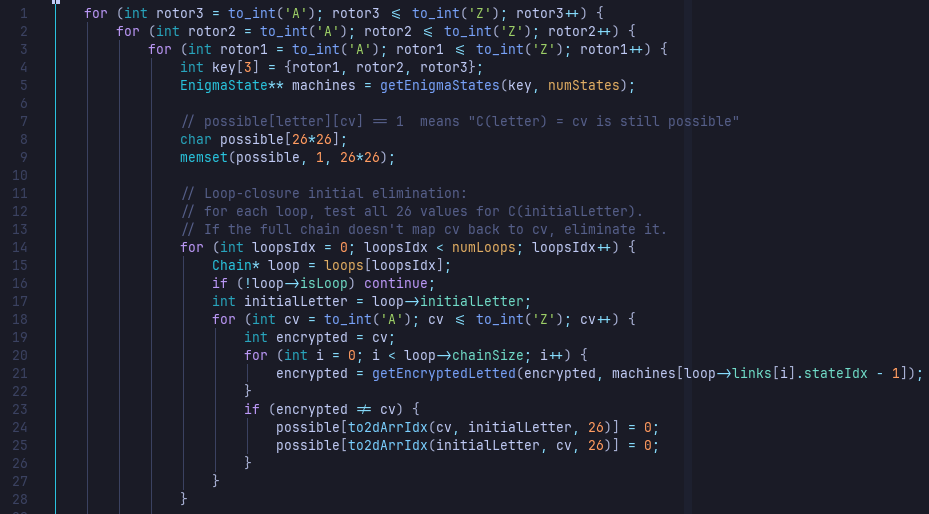
\includegraphics[width=\textwidth]{figures/ex2/loopElimination.png}
        \caption{Elimination of inconsistent loops}\label{fig:loopElimination}
    \end{subfigure}
    ~
    \begin{subfigure}[b]{0.50\textwidth}
        \centering
        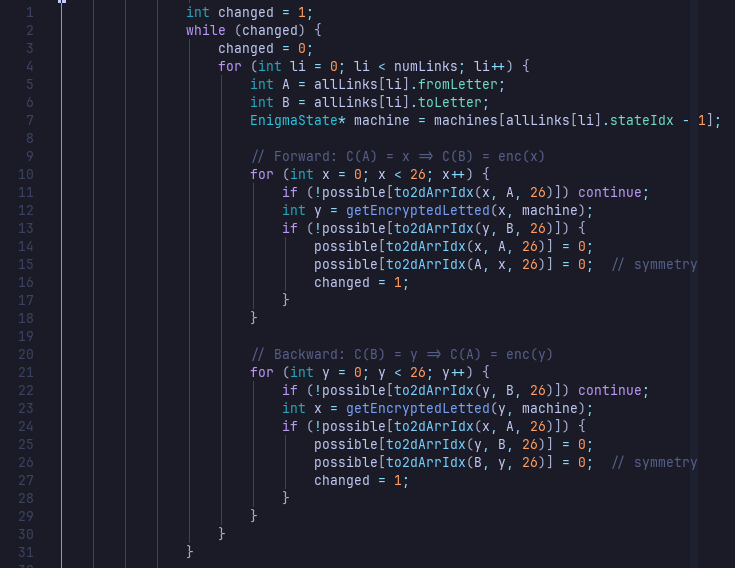
\includegraphics[width=\textwidth]{figures/ex2/welchman.png}
        \caption{Welchan Diagonal Board}\label{fig:welchman}
    \end{subfigure}

    \begin{subfigure}[b]{0.45\textwidth}
        \centering
        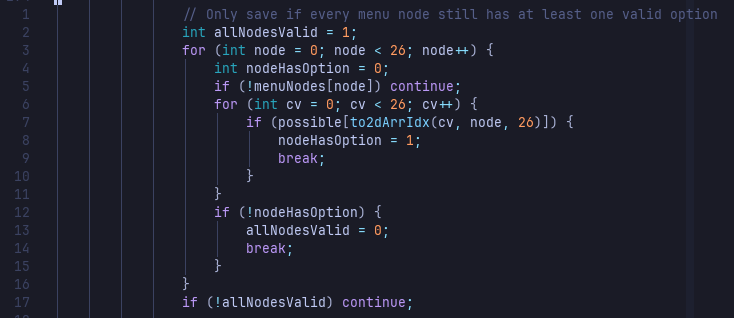
\includegraphics[width=\textwidth]{figures/ex2/potentialKeys.png}
        \caption{Discard Invalid Keys}\label{fig:potentialKeys}
    \end{subfigure}
    ~
    \begin{subfigure}[b]{0.50\textwidth}
        \centering
        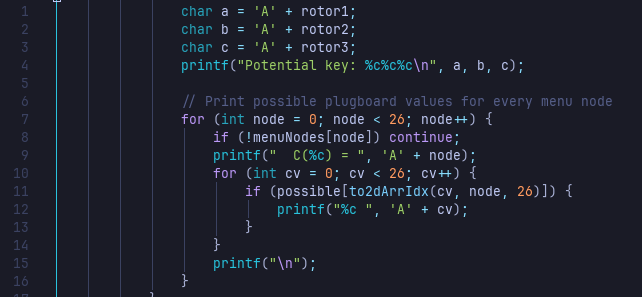
\includegraphics[width=\textwidth]{figures/ex2/finalOutput.png}
        \caption{Final Output}\label{fig:finalOutput}
    \end{subfigure}
\end{figure}

\begin{lstlisting}[language=bash]
$ make ex3 && ./ex3_turing_welchman
gcc ex3_turing_welchman.c -o ex3_turing_welchman
Potential key: RRM
  C(B) = A B G H K N O Q R S U X 
  C(C) = Y 
  C(F) = D E F G H I K L M N U X 
  C(G) = B D E F G H K M R X 
  C(I) = F 
  C(J) = M 
  C(O) = B D E H K L M N Q R W X 
  C(P) = E 
  C(R) = A B G H K N O Q R S U X 
  C(S) = A B D E H K L R U X 
  C(T) = T 
  C(U) = A B E F K L R S U X 
  C(V) = X 
  C(Z) = W 
Potential key: CRR
  C(B) = A B E H K L M N Q R S 
  C(C) = C 
  C(F) = E F K L N O R W Y 
  C(G) = D G H N O U X 
  C(I) = I 
  C(J) = J 
  C(O) = E F G K L O R W Y 
  C(P) = P 
  C(R) = A B E F K L N O Q R Y 
  C(S) = A B D H Q S U 
  C(T) = T 
  C(U) = D G H K S U Y 
  C(V) = V 
  C(Z) = Z 
\end{lstlisting}
From here we can see that we have only $2$ potential keys, and for each key we have a possible plugboard configuration for each letter, which is a significant improvement from the previous method where we had $18$ potential keys and only one possible plugboard configuration per key.

\section{M-209 Collisions}
\subsection{Estimate the probability that the state of the machine repeats at least one time;}
There are $26*25*23*21*19*17 = 101\,405\,850$ possible unique internal states.
With $2000$ messages, each $50$ letters long, a state will occur at every letter encryption, therefore $2\,000 \text{ messages} \times 50 \text{ letters/message} = 100\,000 \text{ total states}$.

To find the number of collisions of these $100'000$ states in the $101'405'850$ possible unique internal states, we can apply the Birthday Paradox:

\begin{align*}
    P(\text{No collisions}) &= \left(\frac{1}{101\,405\,850}\right)^{100\,000} \times (101\,405\,850)^{\underline{100\,000}} \approx 3.79745 \times 10^{-22} \\
    P(\text{At least one collision}) &= 1 - P(\text{No collisions}) \approx 1
\end{align*}

Where $(k)^{\underline{n}}$ represents the falling factorial function.

So it is guaranteed that a collision will eventually happen.
\end{document}
